
%% bare_conf.tex
%% V1.4b
%% 2015/08/26
%% by Michael Shell
%% See:
%% http://www.michaelshell.org/
%% for current contact information.
%%
%% This is a skeleton file demonstrating the use of IEEEtran.cls
%% (requires IEEEtran.cls version 1.8b or later) with an IEEE
%% conference paper.
%%
%% Support sites:
%% http://www.michaelshell.org/tex/ieeetran/
%% http://www.ctan.org/pkg/ieeetran
%% and
%% http://www.ieee.org/

%%*************************************************************************
%% Legal Notice:
%% This code is offered as-is without any warranty either expressed or
%% implied; without even the implied warranty of MERCHANTABILITY or
%% FITNESS FOR A PARTICULAR PURPOSE! 
%% User assumes all risk.
%% In no event shall the IEEE or any contributor to this code be liable for
%% any damages or losses, including, but not limited to, incidental,
%% consequential, or any other damages, resulting from the use or misuse
%% of any information contained here.
%%
%% All comments are the opinions of their respective authors and are not
%% necessarily endorsed by the IEEE.
%%
%% This work is distributed under the LaTeX Project Public License (LPPL)
%% ( http://www.latex-project.org/ ) version 1.3, and may be freely used,
%% distributed and modified. A copy of the LPPL, version 1.3, is included
%% in the base LaTeX documentation of all distributions of LaTeX released
%% 2003/12/01 or later.
%% Retain all contribution notices and credits.
%% ** Modified files should be clearly indicated as such, including  **
%% ** renaming them and changing author support contact information. **
%%*************************************************************************


% *** Authors should verify (and, if needed, correct) their LaTeX system  ***
% *** with the testflow diagnostic prior to trusting their LaTeX platform ***
% *** with production work. The IEEE's font choices and paper sizes can   ***
% *** trigger bugs that do not appear when using other class files.       ***                          ***
% The testflow support page is at:
% http://www.michaelshell.org/tex/testflow/



\documentclass[conference]{IEEEtran}
% Some Computer Society conferences also require the compsoc mode option,
% but others use the standard conference format.
%
% If IEEEtran.cls has not been installed into the LaTeX system files,
% manually specify the path to it like:
% \documentclass[conference]{../sty/IEEEtran}





% Some very useful LaTeX packages include:
% (uncomment the ones you want to load)


% *** MISC UTILITY PACKAGES ***
%
%\usepackage{ifpdf}
% Heiko Oberdiek's ifpdf.sty is very useful if you need conditional
% compilation based on whether the output is pdf or dvi.
% usage:
% \ifpdf
%   % pdf code
% \else
%   % dvi code
% \fi
% The latest version of ifpdf.sty can be obtained from:
% http://www.ctan.org/pkg/ifpdf
% Also, note that IEEEtran.cls V1.7 and later provides a builtin
% \ifCLASSINFOpdf conditional that works the same way.
% When switching from latex to pdflatex and vice-versa, the compiler may
% have to be run twice to clear warning/error messages.






% *** CITATION PACKAGES ***
%
%\usepackage{cite}
% cite.sty was written by Donald Arseneau
% V1.6 and later of IEEEtran pre-defines the format of the cite.sty package
% \cite{} output to follow that of the IEEE. Loading the cite package will
% result in citation numbers being automatically sorted and properly
% "compressed/ranged". e.g., [1], [9], [2], [7], [5], [6] without using
% cite.sty will become [1], [2], [5]--[7], [9] using cite.sty. cite.sty's
% \cite will automatically add leading space, if needed. Use cite.sty's
% noadjust option (cite.sty V3.8 and later) if you want to turn this off
% such as if a citation ever needs to be enclosed in parenthesis.
% cite.sty is already installed on most LaTeX systems. Be sure and use
% version 5.0 (2009-03-20) and later if using hyperref.sty.
% The latest version can be obtained at:
% http://www.ctan.org/pkg/cite
% The documentation is contained in the cite.sty file itself.






% *** GRAPHICS RELATED PACKAGES ***
%
\ifCLASSINFOpdf
  % \usepackage[pdftex]{graphicx}
  % declare the path(s) where your graphic files are
  % \graphicspath{{../pdf/}{../jpeg/}}
  % and their extensions so you won't have to specify these with
  % every instance of \includegraphics
  % \DeclareGraphicsExtensions{.pdf,.jpeg,.png}
\else
  % or other class option (dvipsone, dvipdf, if not using dvips). graphicx
  % will default to the driver specified in the system graphics.cfg if no
  % driver is specified.
  % \usepackage[dvips]{graphicx}
  % declare the path(s) where your graphic files are
  % \graphicspath{{../eps/}}
  % and their extensions so you won't have to specify these with
  % every instance of \includegraphics
  % \DeclareGraphicsExtensions{.eps}
\fi
% graphicx was written by David Carlisle and Sebastian Rahtz. It is
% required if you want graphics, photos, etc. graphicx.sty is already
% installed on most LaTeX systems. The latest version and documentation
% can be obtained at: 
% http://www.ctan.org/pkg/graphicx
% Another good source of documentation is "Using Imported Graphics in
% LaTeX2e" by Keith Reckdahl which can be found at:
% http://www.ctan.org/pkg/epslatex
%
% latex, and pdflatex in dvi mode, support graphics in encapsulated
% postscript (.eps) format. pdflatex in pdf mode supports graphics
% in .pdf, .jpeg, .png and .mps (metapost) formats. Users should ensure
% that all non-photo figures use a vector format (.eps, .pdf, .mps) and
% not a bitmapped formats (.jpeg, .png). The IEEE frowns on bitmapped formats
% which can result in "jaggedy"/blurry rendering of lines and letters as
% well as large increases in file sizes.
%
% You can find documentation about the pdfTeX application at:
% http://www.tug.org/applications/pdftex





% *** MATH PACKAGES ***
%
%\usepackage{amsmath}
% A popular package from the American Mathematical Society that provides
% many useful and powerful commands for dealing with mathematics.
%
% Note that the amsmath package sets \interdisplaylinepenalty to 10000
% thus preventing page breaks from occurring within multiline equations. Use:
%\interdisplaylinepenalty=2500
% after loading amsmath to restore such page breaks as IEEEtran.cls normally
% does. amsmath.sty is already installed on most LaTeX systems. The latest
% version and documentation can be obtained at:
% http://www.ctan.org/pkg/amsmath





% *** SPECIALIZED LIST PACKAGES ***
%
%\usepackage{algorithmic}
% algorithmic.sty was written by Peter Williams and Rogerio Brito.
% This package provides an algorithmic environment fo describing algorithms.
% You can use the algorithmic environment in-text or within a figure
% environment to provide for a floating algorithm. Do NOT use the algorithm
% floating environment provided by algorithm.sty (by the same authors) or
% algorithm2e.sty (by Christophe Fiorio) as the IEEE does not use dedicated
% algorithm float types and packages that provide these will not provide
% correct IEEE style captions. The latest version and documentation of
% algorithmic.sty can be obtained at:
% http://www.ctan.org/pkg/algorithms
% Also of interest may be the (relatively newer and more customizable)
% algorithmicx.sty package by Szasz Janos:
% http://www.ctan.org/pkg/algorithmicx




% *** ALIGNMENT PACKAGES ***
%
%\usepackage{array}
% Frank Mittelbach's and David Carlisle's array.sty patches and improves
% the standard LaTeX2e array and tabular environments to provide better
% appearance and additional user controls. As the default LaTeX2e table
% generation code is lacking to the point of almost being broken with
% respect to the quality of the end results, all users are strongly
% advised to use an enhanced (at the very least that provided by array.sty)
% set of table tools. array.sty is already installed on most systems. The
% latest version and documentation can be obtained at:
% http://www.ctan.org/pkg/array


% IEEEtran contains the IEEEeqnarray family of commands that can be used to
% generate multiline equations as well as matrices, tables, etc., of high
% quality.




% *** SUBFIGURE PACKAGES ***
%\ifCLASSOPTIONcompsoc
%  \usepackage[caption=false,font=normalsize,labelfont=sf,textfont=sf]{subfig}
%\else
%  \usepackage[caption=false,font=footnotesize]{subfig}
%\fi
% subfig.sty, written by Steven Douglas Cochran, is the modern replacement
% for subfigure.sty, the latter of which is no longer maintained and is
% incompatible with some LaTeX packages including fixltx2e. However,
% subfig.sty requires and automatically loads Axel Sommerfeldt's caption.sty
% which will override IEEEtran.cls' handling of captions and this will result
% in non-IEEE style figure/table captions. To prevent this problem, be sure
% and invoke subfig.sty's "caption=false" package option (available since
% subfig.sty version 1.3, 2005/06/28) as this is will preserve IEEEtran.cls
% handling of captions.
% Note that the Computer Society format requires a larger sans serif font
% than the serif footnote size font used in traditional IEEE formatting
% and thus the need to invoke different subfig.sty package options depending
% on whether compsoc mode has been enabled.
%
% The latest version and documentation of subfig.sty can be obtained at:
% http://www.ctan.org/pkg/subfig




% *** FLOAT PACKAGES ***
%
%\usepackage{fixltx2e}
% fixltx2e, the successor to the earlier fix2col.sty, was written by
% Frank Mittelbach and David Carlisle. This package corrects a few problems
% in the LaTeX2e kernel, the most notable of which is that in current
% LaTeX2e releases, the ordering of single and double column floats is not
% guaranteed to be preserved. Thus, an unpatched LaTeX2e can allow a
% single column figure to be placed prior to an earlier double column
% figure.
% Be aware that LaTeX2e kernels dated 2015 and later have fixltx2e.sty's
% corrections already built into the system in which case a warning will
% be issued if an attempt is made to load fixltx2e.sty as it is no longer
% needed.
% The latest version and documentation can be found at:
% http://www.ctan.org/pkg/fixltx2e


%\usepackage{stfloats}
% stfloats.sty was written by Sigitas Tolusis. This package gives LaTeX2e
% the ability to do double column floats at the bottom of the page as well
% as the top. (e.g., "\begin{figure*}[!b]" is not normally possible in
% LaTeX2e). It also provides a command:
%\fnbelowfloat
% to enable the placement of footnotes below bottom floats (the standard
% LaTeX2e kernel puts them above bottom floats). This is an invasive package
% which rewrites many portions of the LaTeX2e float routines. It may not work
% with other packages that modify the LaTeX2e float routines. The latest
% version and documentation can be obtained at:
% http://www.ctan.org/pkg/stfloats
% Do not use the stfloats baselinefloat ability as the IEEE does not allow
% \baselineskip to stretch. Authors submitting work to the IEEE should note
% that the IEEE rarely uses double column equations and that authors should try
% to avoid such use. Do not be tempted to use the cuted.sty or midfloat.sty
% packages (also by Sigitas Tolusis) as the IEEE does not format its papers in
% such ways.
% Do not attempt to use stfloats with fixltx2e as they are incompatible.
% Instead, use Morten Hogholm'a dblfloatfix which combines the features
% of both fixltx2e and stfloats:
%
% \usepackage{dblfloatfix}
% The latest version can be found at:
% http://www.ctan.org/pkg/dblfloatfix




% *** PDF, URL AND HYPERLINK PACKAGES ***
%
%\usepackage{url}
% url.sty was written by Donald Arseneau. It provides better support for
% handling and breaking URLs. url.sty is already installed on most LaTeX
% systems. The latest version and documentation can be obtained at:
% http://www.ctan.org/pkg/url
% Basically, \url{my_url_here}.




% *** Do not adjust lengths that control margins, column widths, etc. ***
% *** Do not use packages that alter fonts (such as pslatex).         ***
% There should be no need to do such things with IEEEtran.cls V1.6 and later.
% (Unless specifically asked to do so by the journal or conference you plan
% to submit to, of course. )


% correct bad hyphenation here
\hyphenation{op-tical net-works semi-conduc-tor}
\usepackage{graphicx}
\graphicspath{ {./draft_outputs/} }

\begin{document}
%
% paper title
% Titles are generally capitalized except for words such as a, an, and, as,
% at, but, by, for, in, nor, of, on, or, the, to and up, which are usually
% not capitalized unless they are the first or last word of the title.
% Linebreaks \\ can be used within to get better formatting as desired.
% Do not put math or special symbols in the title.
\title{CMSC733 Project 1: MyAutoPano}


% author names and affiliations
% use a multiple column layout for up to three different
% affiliations
\author{\IEEEauthorblockN{Ha Phan Nguyen}
\IEEEauthorblockA{
University of Maryland, College Park\\
Email: phan2003@umd.edu}
\and
\IEEEauthorblockN{Hengyi Wu}
\IEEEauthorblockA{University of Maryland, College Park\\
Email: hw987@umd.edu}
}

% conference papers do not typically use \thanks and this command
% is locked out in conference mode. If really needed, such as for
% the acknowledgment of grants, issue a \IEEEoverridecommandlockouts
% after \documentclass

% for over three affiliations, or if they all won't fit within the width
% of the page, use this alternative format:
% 
%\author{\IEEEauthorblockN{Michael Shell\IEEEauthorrefmark{1},
%Homer Simpson\IEEEauthorrefmark{2},
%James Kirk\IEEEauthorrefmark{3}, 
%Montgomery Scott\IEEEauthorrefmark{3} and
%Eldon Tyrell\IEEEauthorrefmark{4}}
%\IEEEauthorblockA{\IEEEauthorrefmark{1}School of Electrical and Computer Engineering\\
%Georgia Institute of Technology,
%Atlanta, Georgia 30332--0250\\ Email: see http://www.michaelshell.org/contact.html}
%\IEEEauthorblockA{\IEEEauthorrefmark{2}Twentieth Century Fox, Springfield, USA\\
%Email: homer@thesimpsons.com}
%\IEEEauthorblockA{\IEEEauthorrefmark{3}Starfleet Academy, San Francisco, California 96678-2391\\
%Telephone: (800) 555--1212, Fax: (888) 555--1212}
%\IEEEauthorblockA{\IEEEauthorrefmark{4}Tyrell Inc., 123 Replicant Street, Los Angeles, California 90210--4321}}




% use for special paper notices
%\IEEEspecialpapernotice{(Invited Paper)}




% make the title area
\maketitle

% As a general rule, do not put math, special symbols or citations
% in the abstract
\begin{abstract}
This report goes over the various panorama stitching techniques 
discussed in the course project. We go over the methodology, 
ideas, and implementation of stitching techniques. In phase 1,
we use a traditional feature-matching approach to stitching. In
Phase 2, we implement supervised and unsupervised deep learning
 approaches to estimate the homography between two images and
 blend them.
\end{abstract}

% no keywords




% For peer review papers, you can put extra information on the cover
% page as needed:
% \ifCLASSOPTIONpeerreview
% \begin{center} \bfseries EDICS Category: 3-BBND \end{center}
% \fi
%
% For peerreview papers, this IEEEtran command inserts a page break and
% creates the second title. It will be ignored for other modes.
\IEEEpeerreviewmaketitle



\section{Phase 1}

In this implementation, we first resize the input images down to a maximum width of 
800 pixels as an optimization for memory. Each image is then projected on a cylinder
using an estimated focal length. Then, we used Harris Corner to get corners of all
images and then select 3000 best corners that are uniformly distributed. We then 
extracted the feature locations to feature vectors according to the project's 
specifications, and then compared these vectors to adjacent images to get the best
match distances. We then calculate the homography matrix next and then test this 
matrix against all other matches, keeping the transformation that yields the 
highest number of inliers. We then use the middle image as the reference then chain
all other homography matrices to map images onto the middle image. We do alpha blending
to smooth the images.

\subsection{Preprocessing}
We begin preprocessing by reading the images and resizing them 
so their maximum width is capped at 800 pixels, scaling the height proportionally 
to optimize for memory. After resizing, the images undergo cylindrical 
projection via the helper.cylindrical\_warp function. This function approximates 
the camera's focal length as the image's width and performs an inverse mapping 
technique. It calculates where each pixel on a 2D plane would mathematically 
sit on a cylinder using tangent and cosine functions, and then reconstructs 
the warped image using OpenCV's remap function. This is needed to avoid extreme
distortions in cases where a multitude of images need to be stitched.

\begin{figure}[!t]
\centering
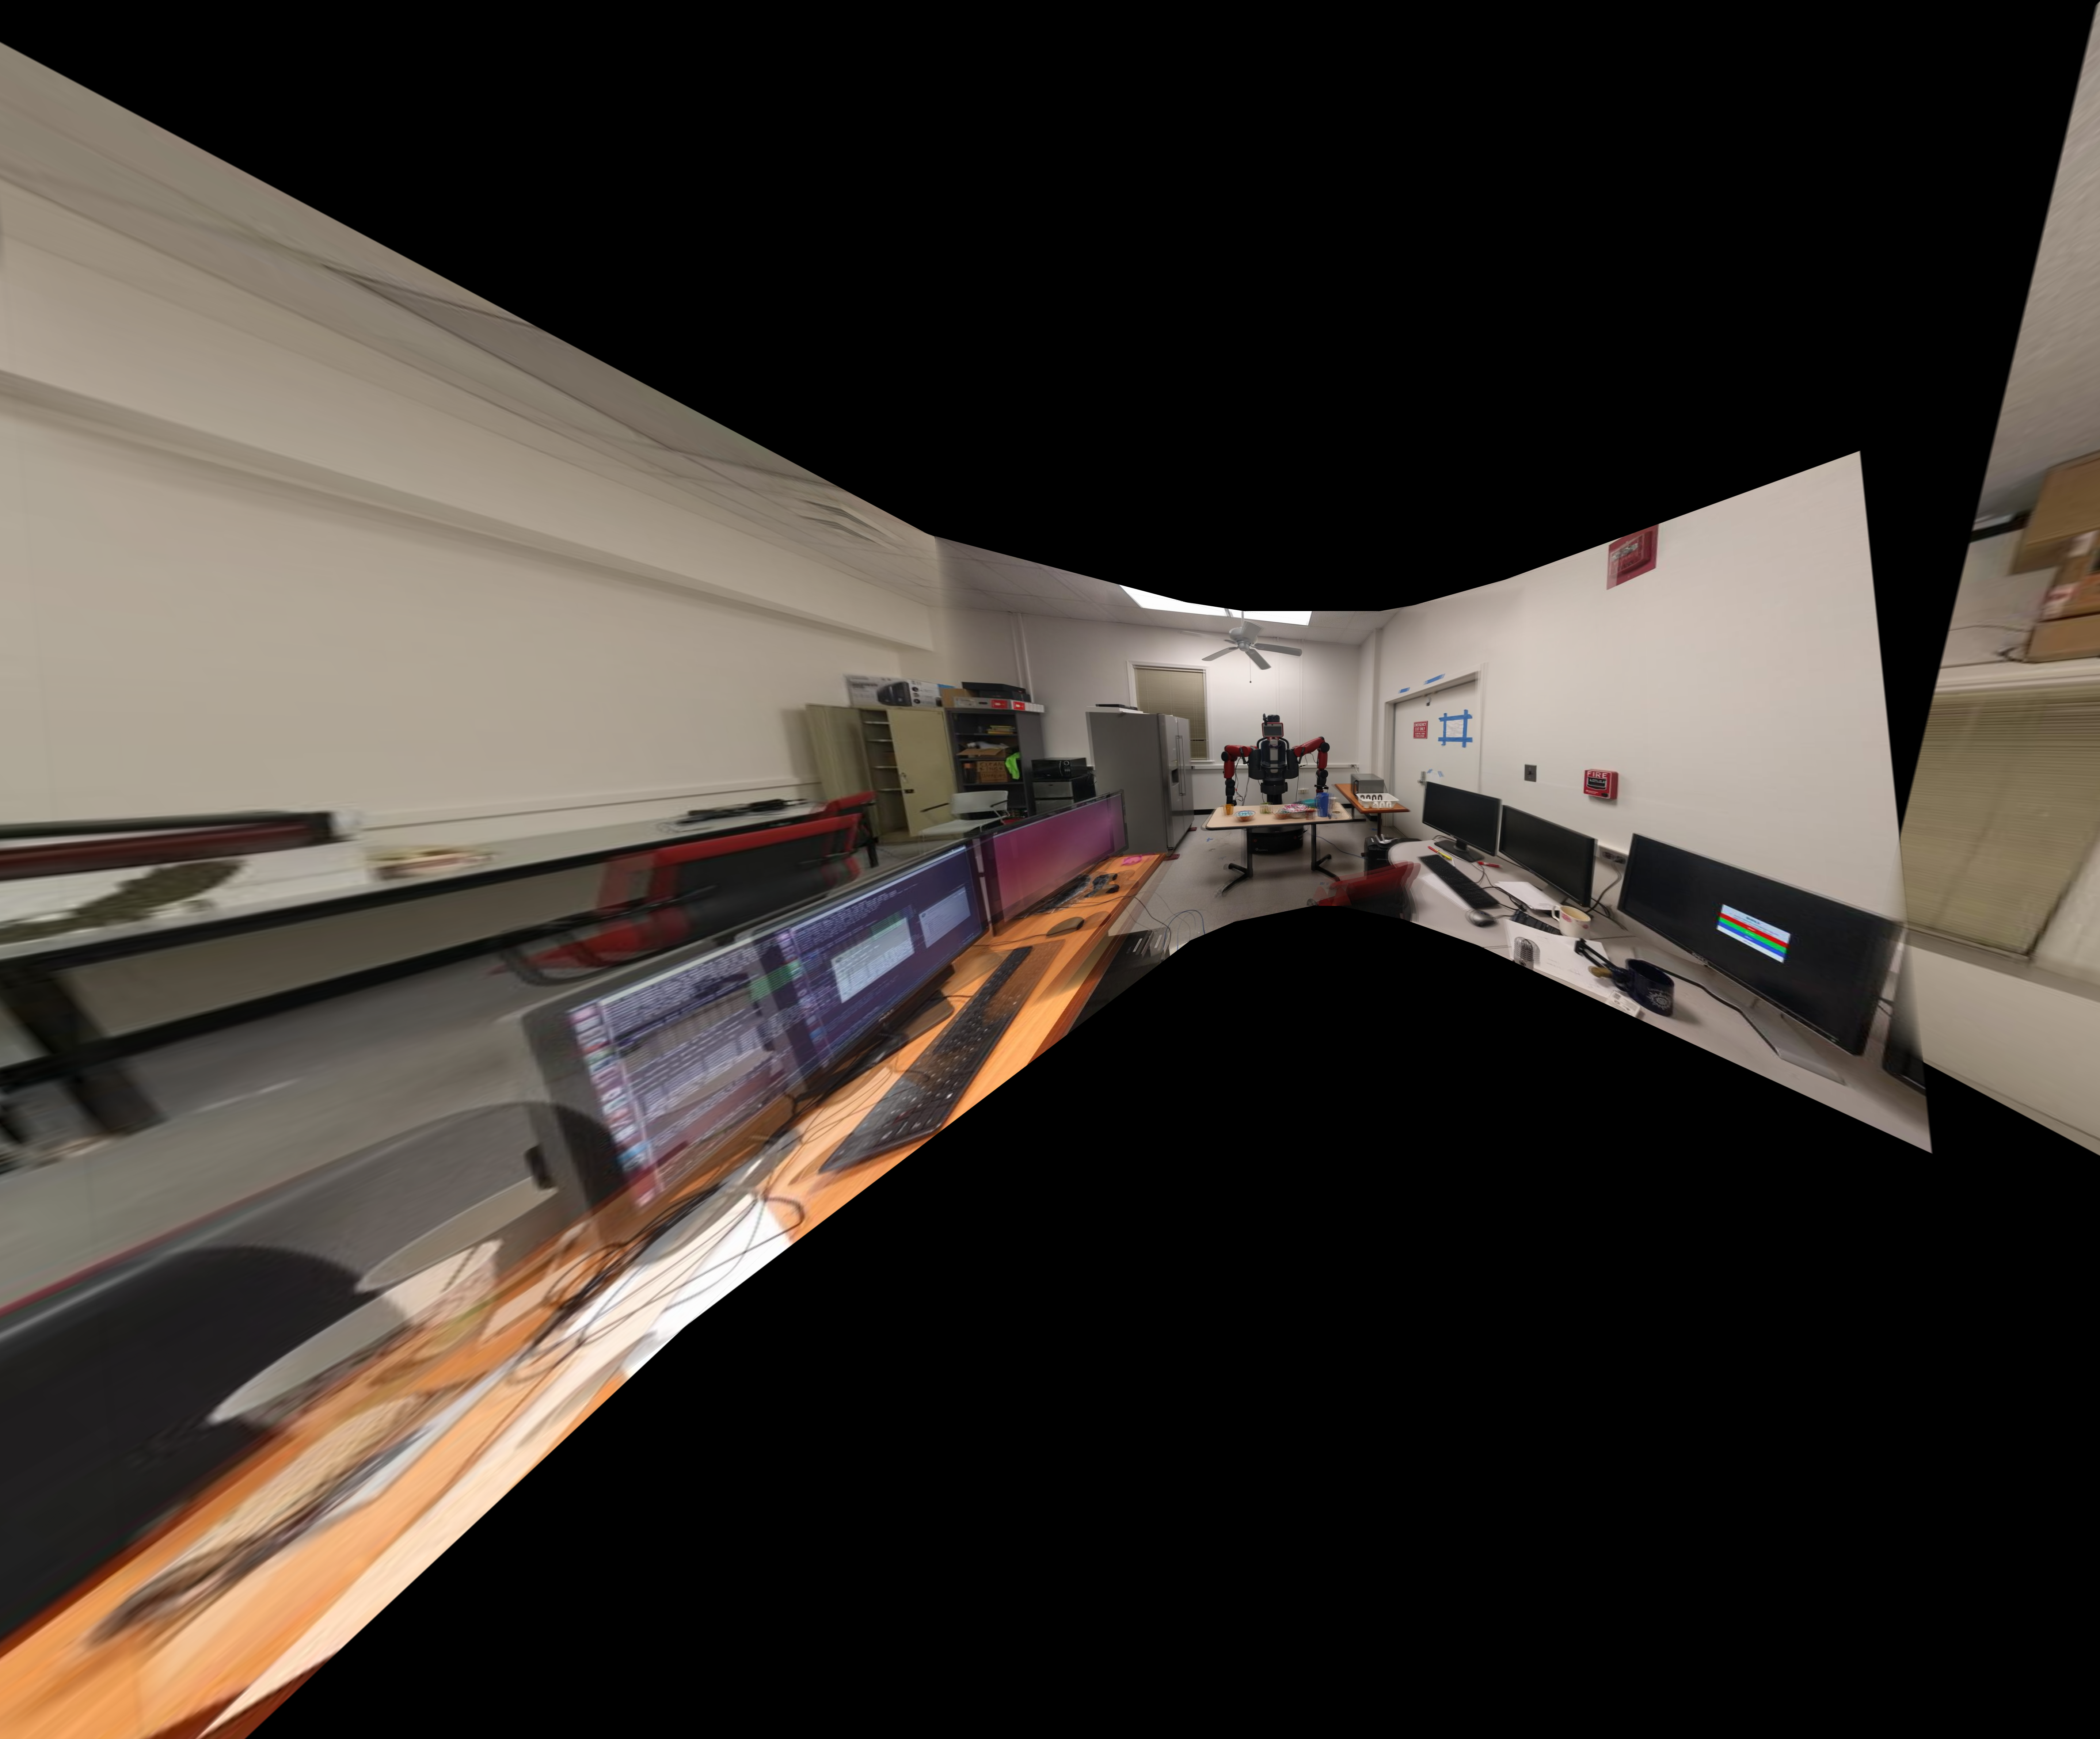
\includegraphics[width=\linewidth]{set3_feather.png}
\caption{Stitching without cylindrical warp.}
\label{fig_example}
\end{figure}

\subsection{Corner Detection}
Corner detection is implemented using OpenCV's Harris Corner method. This function computes a corner 
response score for each pixel, utilizing a neighborhood block size of 2, a Sobel 
derivative kernel size of 3, and a Harris free parameter of 0.04. For visualization, 
pixels that have a response core exceeding 1\% of the maximum score in the image are 
isolated, highlighted in red on a copy of the original image, and saved to the output 
directory.

\begin{figure}[!t]
\centering
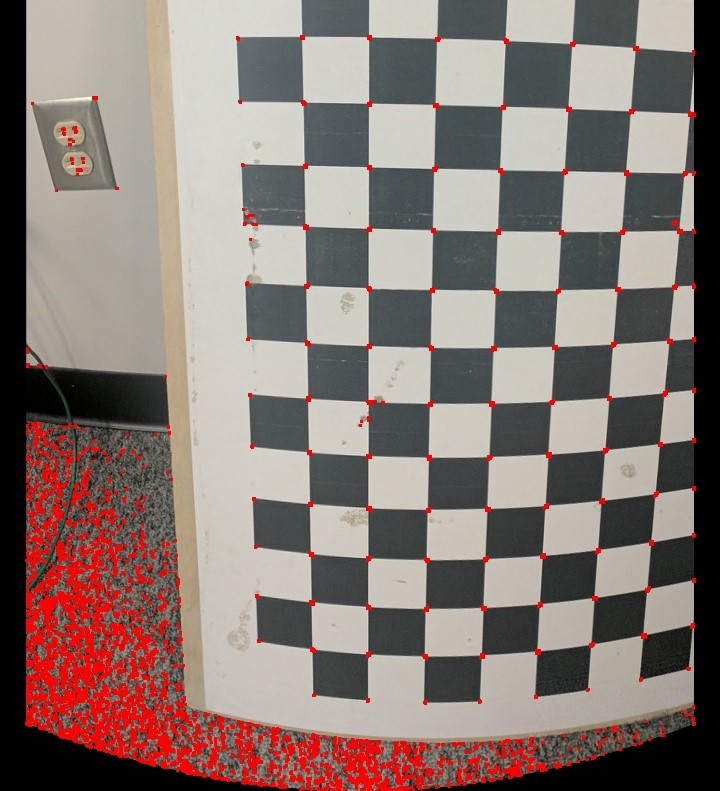
\includegraphics[width=\linewidth]{corners_1.jpg}
\caption{Corner locations image by the Harris Corner function}
\label{fig_example}
\end{figure}


\subsection{AMNS}
The ANMS step takes the Harris corners and identifying local maxima using the 
peak\_local\_max function to gather a baseline set of strong corner candidates. For each 
candidate, the algorithm calculates the minimum Euclidean distance to any other corner 
that has a strictly higher response score. By sorting these radii in 
descending order and selecting the top N\_best points, this prevents the algorithm 
from clustering all its keypoints in a single highly textured region, which is important 
for later image stitching.

\subsection{Feature Descriptors and Matching}
The code iterates through the ANMS keypoints and extracts a 40x40 pixel patch around 
each point. We then uses reflection padding to handle points near the edges. Each patch 
is then smoothed with Gaussian blur and sub-sampled. Finally, the resulting grid is flattened 
into a 64-dimensional vector and standardized to have a mean of zero and a variance of 
one.
Each feature vector is compared between images using SSD. For a given feature 
in the first image, the algorithm computes the SSD against all features in the second 
image to find the absolute closest and second-closest matches. A match is only accepted if the 
distance to the best match is less than the value ratio\_thresh of the distance to the 
second-best match. 

\begin{figure}[!t]
\centering
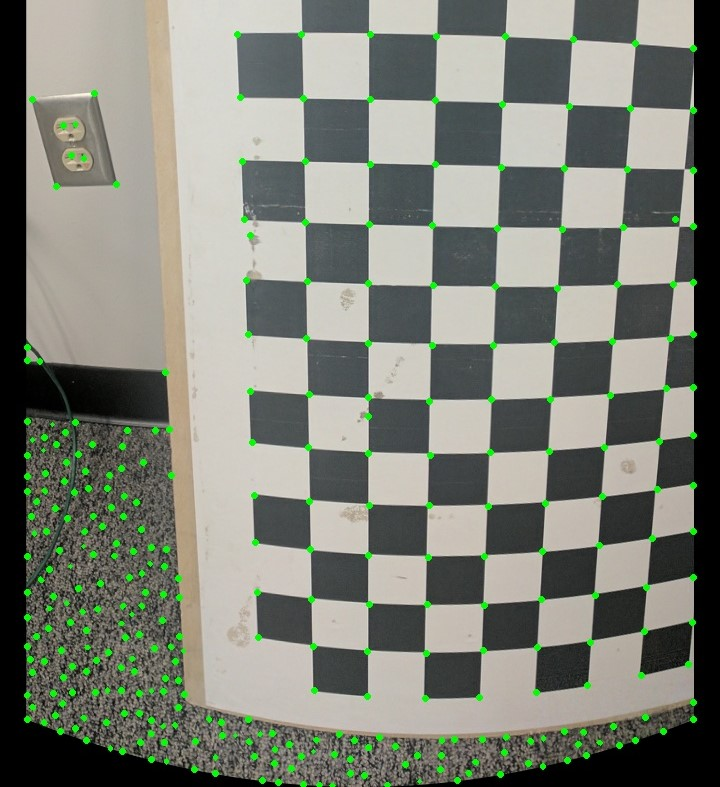
\includegraphics[width=\linewidth]{anms_1.jpg}
\caption{Choosing N\_best corners using AMNS}
\label{fig_example2}
\end{figure}

\begin{figure}[!t]
\centering
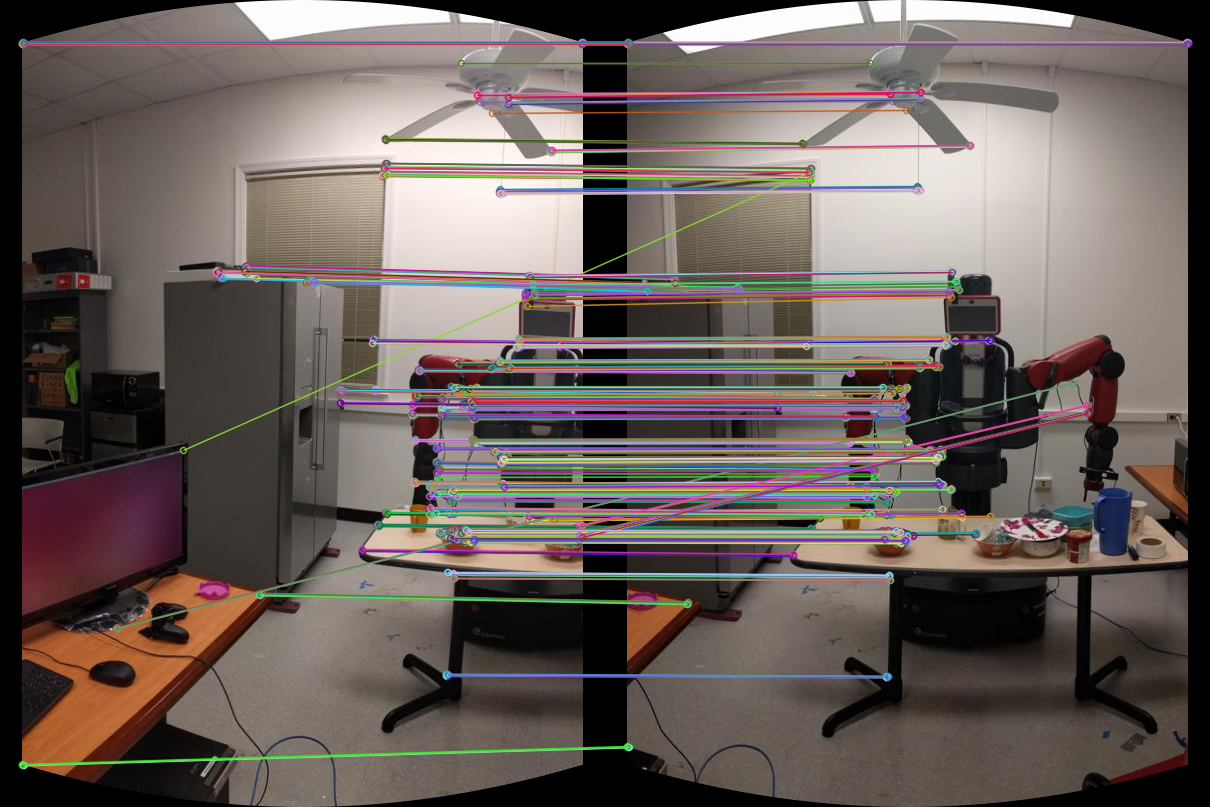
\includegraphics[width=\linewidth]{matching.png}
\caption{Matching features between images}
\label{fig_example2}
\end{figure}

\subsection{RANSAC}
RANSAC is used to find the best homography from one image to another.
Through a number of iterations, we randomly select four pairs of matched keypoints and 
calculates a Homography matrix, based on these points. The algorithm then applies this 
matrix to all the matched points from the first image,  projecting them into the 
coordinate space of the second image. It calculates the SSD 
between newly projected coordinates and their actual matched locations. If the 
distance is below a fixed value named tau, the pair is classified as inliers.

After testing a large number of matrices, the algorithm identifies the matrix that produced 
the largest consensus set of inlier pairs. Then, all outliers are discarded and we
recalculate an optimized Homography matrix using cv.findHomography on every 
single verified inlier.

\begin{figure}[!t]
\centering
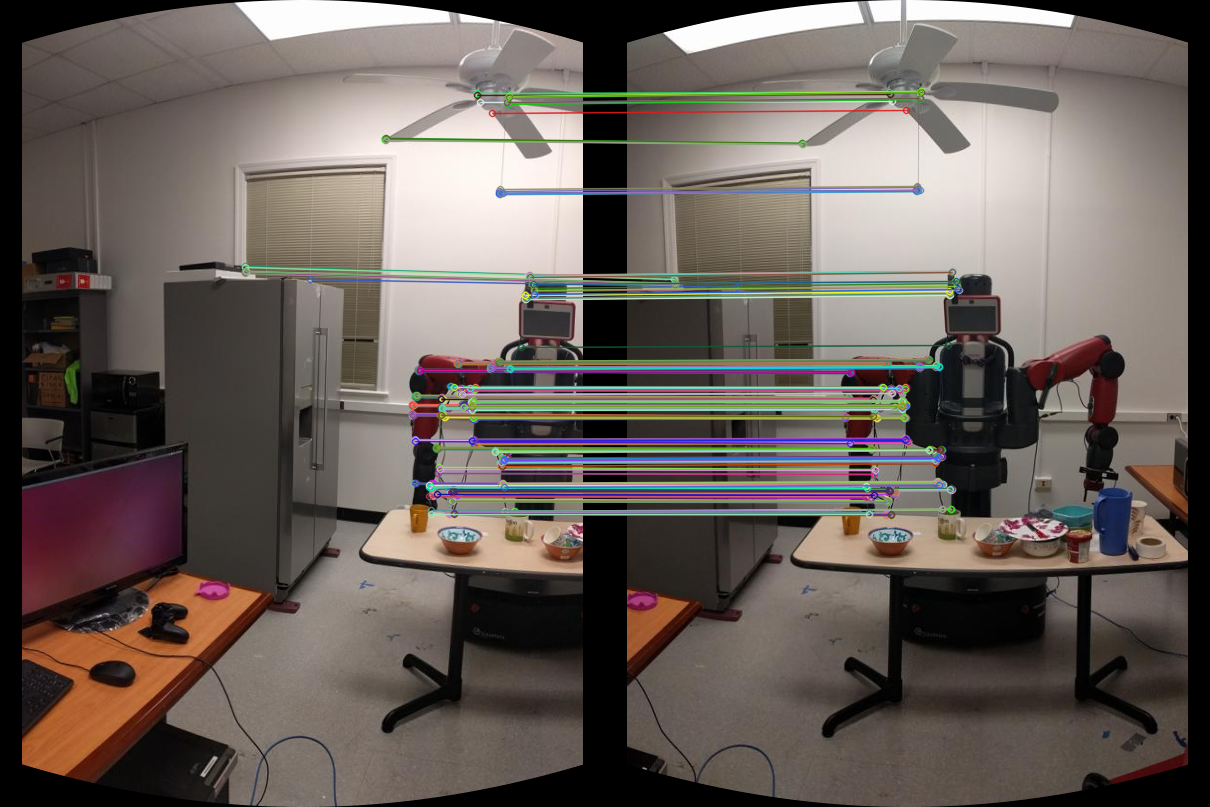
\includegraphics[width=\linewidth]{ransac.png}
\caption{Eliminating bad feature pairs and calculate homography using RANSAC }
\label{fig_example2}
\end{figure}

\subsection{Warping and Blending}
The middle image of the sequence is chosen as the fixed reference frame. We then chain 
the pairwise homography matrices together to compute a global homography for every other 
image. Next, it calculates the outer bounding box of all these transformed images to 
determine the final canvas size and creates a global translation matrix to shift everything 
into correct coordinates.

To stitch overlapping regions, we use a Distance Transform blending technique. 
For every warped image, it generates a binary mask and calculates how 
far each pixel is from the image's boundary.  These distances are normalized and used as 
alpha weights. Pixels near the center of an original image stay in the panorama, while pixels 
near the edges fade out. All the weighted images are accumulated into a floating-point array 
and then divided by the total weight map to produce the blended panorama.

The Poisson Blending technique was considered, but the final output became much darker
than the original images.

\begin{figure}[!t]
\centering
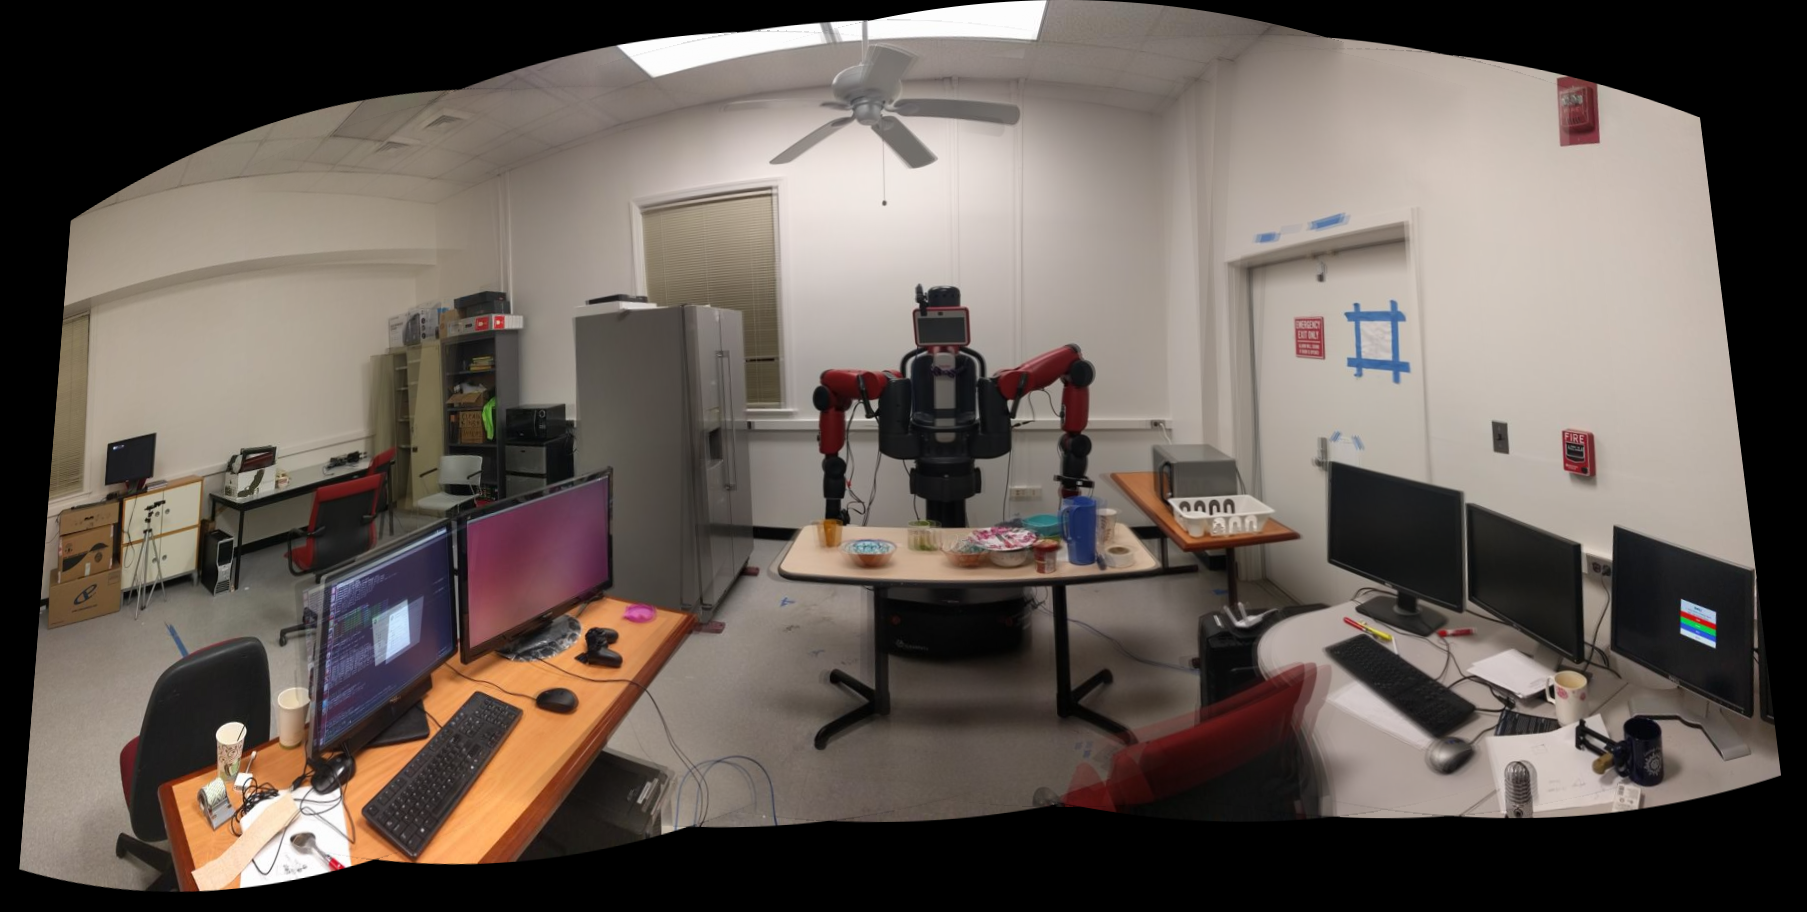
\includegraphics[width=\linewidth]{set3_feather_cylindrical.png}
\caption{Final panorama with cylindrical warp of train set 3.}
\label{fig_example}
\end{figure}

\begin{figure}[!t]
\centering
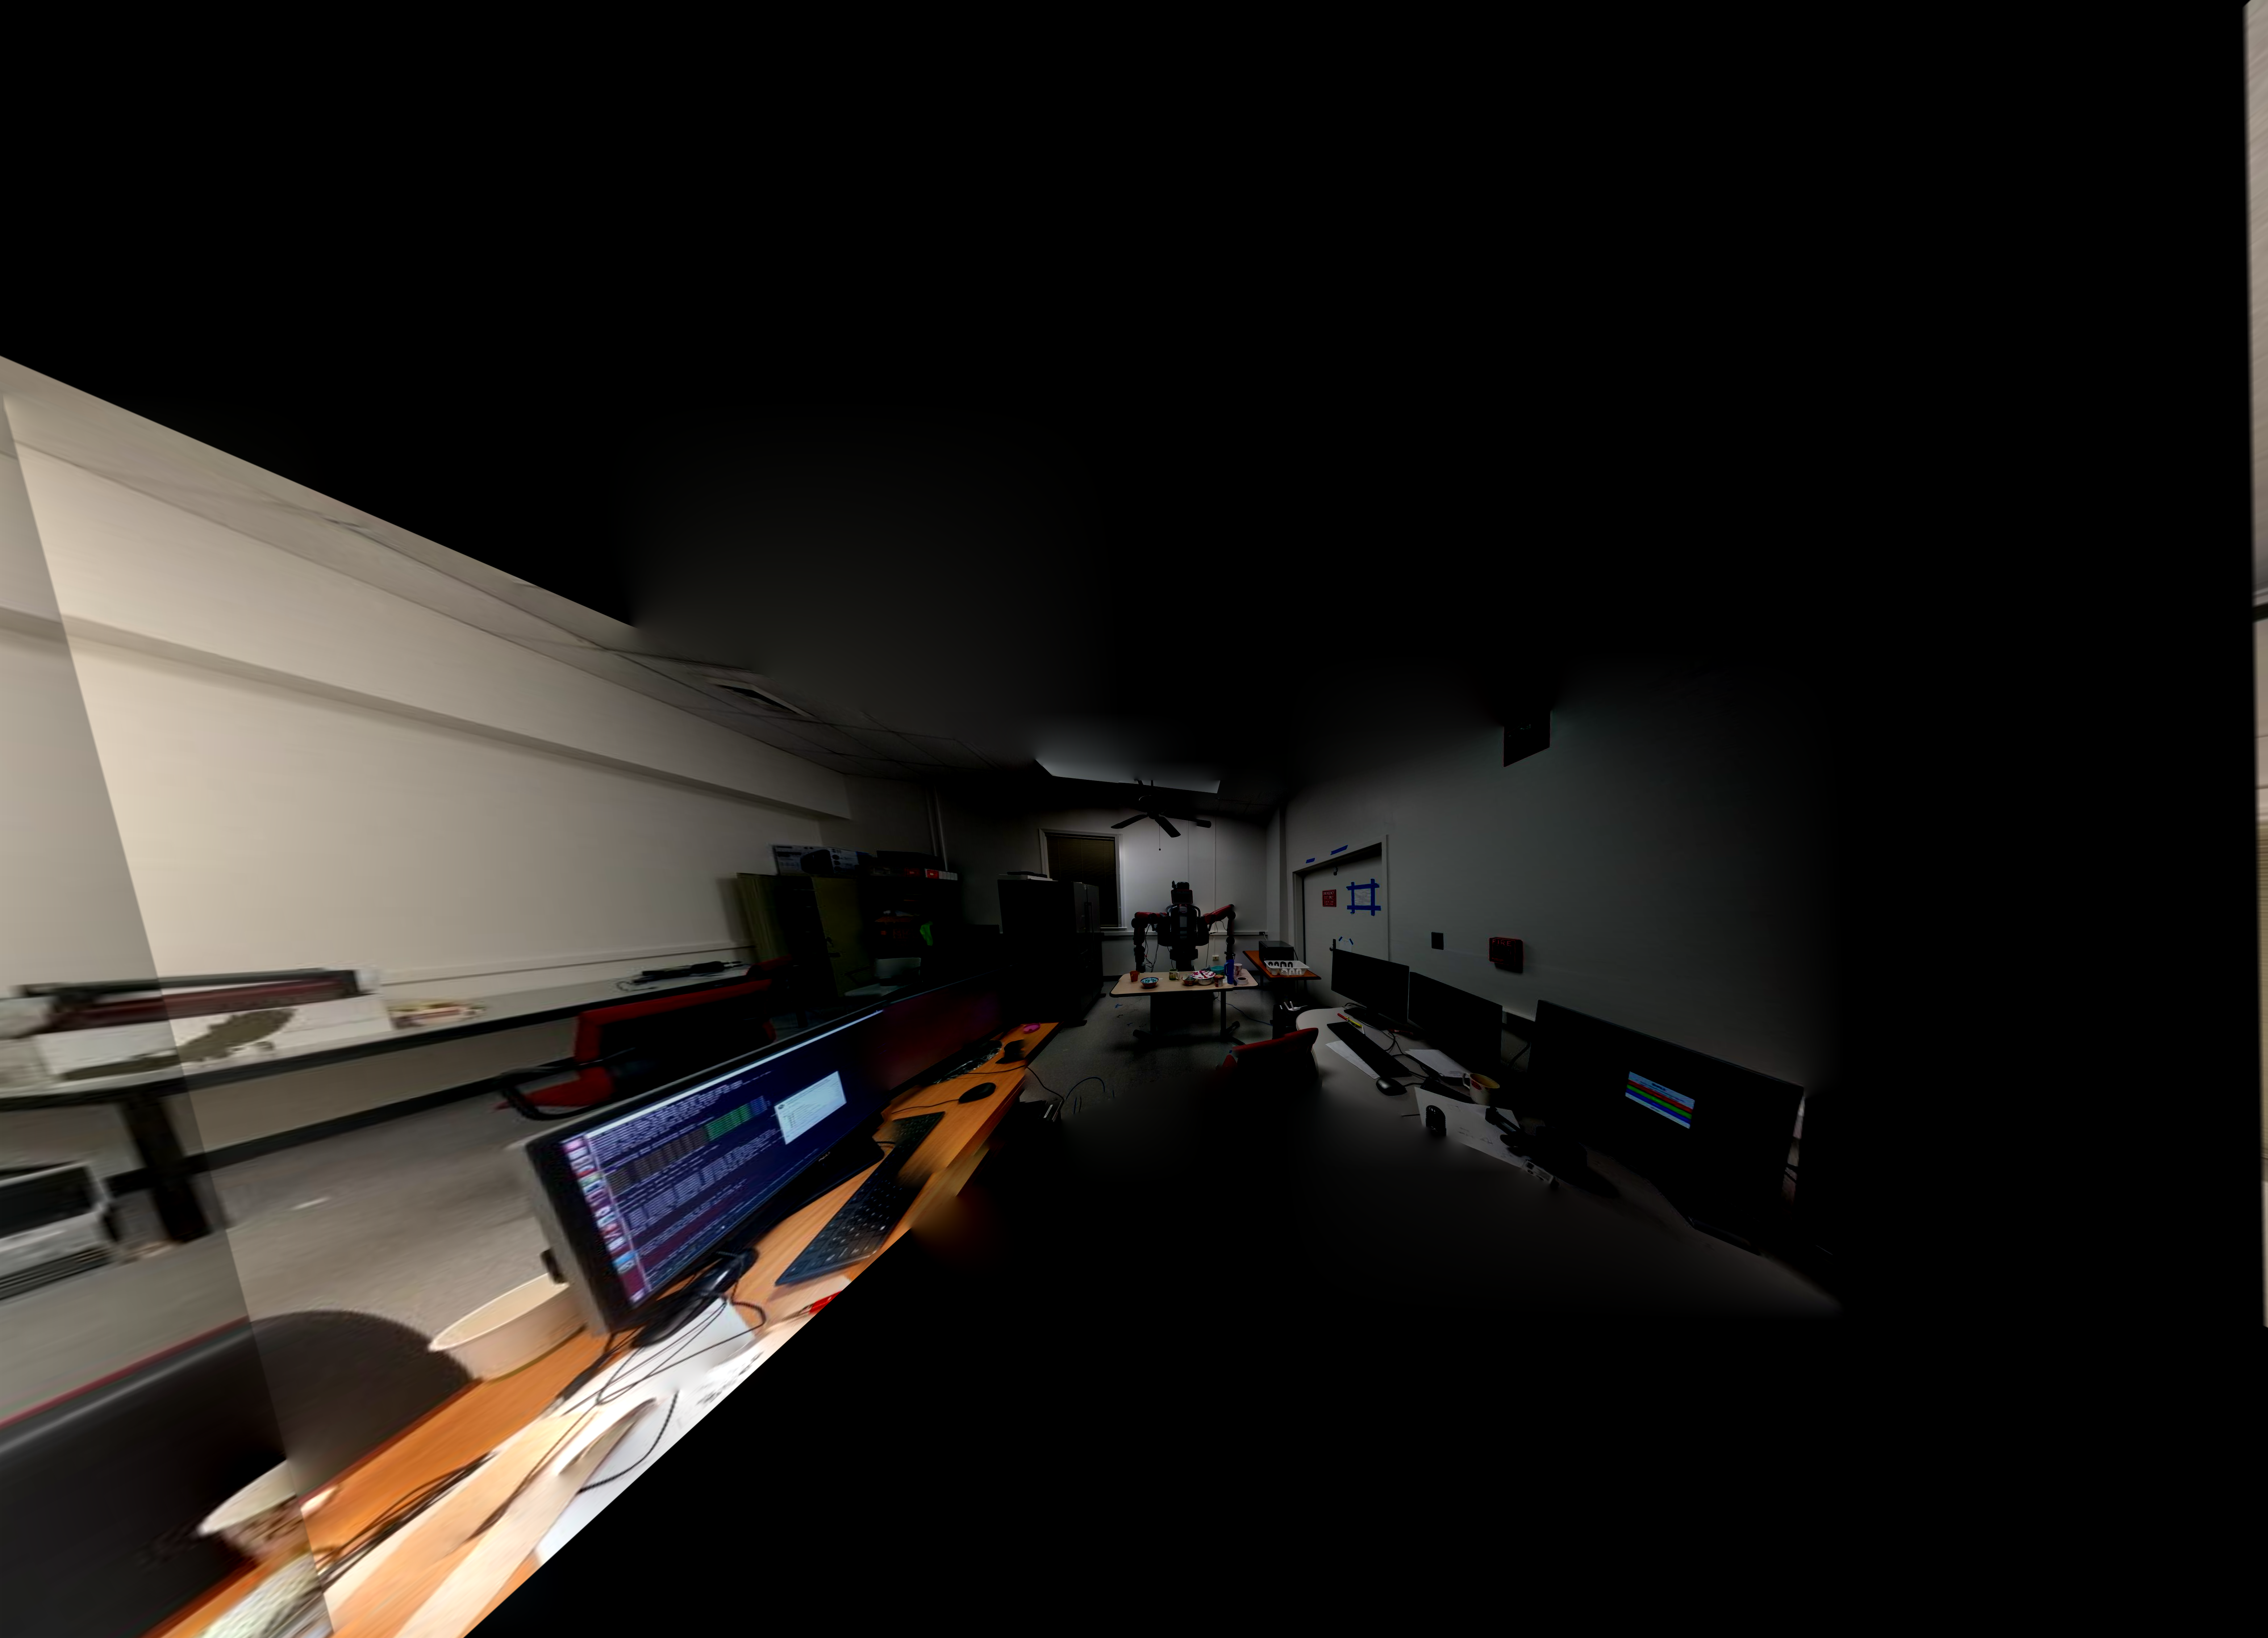
\includegraphics[width=\linewidth]{set3_poisson_mypano.png}
\caption{Poisson blending darkens the final panorama}
\label{fig_example}
\end{figure}

\subsection{Handling low/no overlap}
At the start of feature matching, we defined a hard threshold where for two images to be 
considered overlapping, they must share at least a fixed number of inliers from RANSAC to be 
considered in the final panorama. This is set to 60 as a default.

\begin{figure}[!t]
\centering
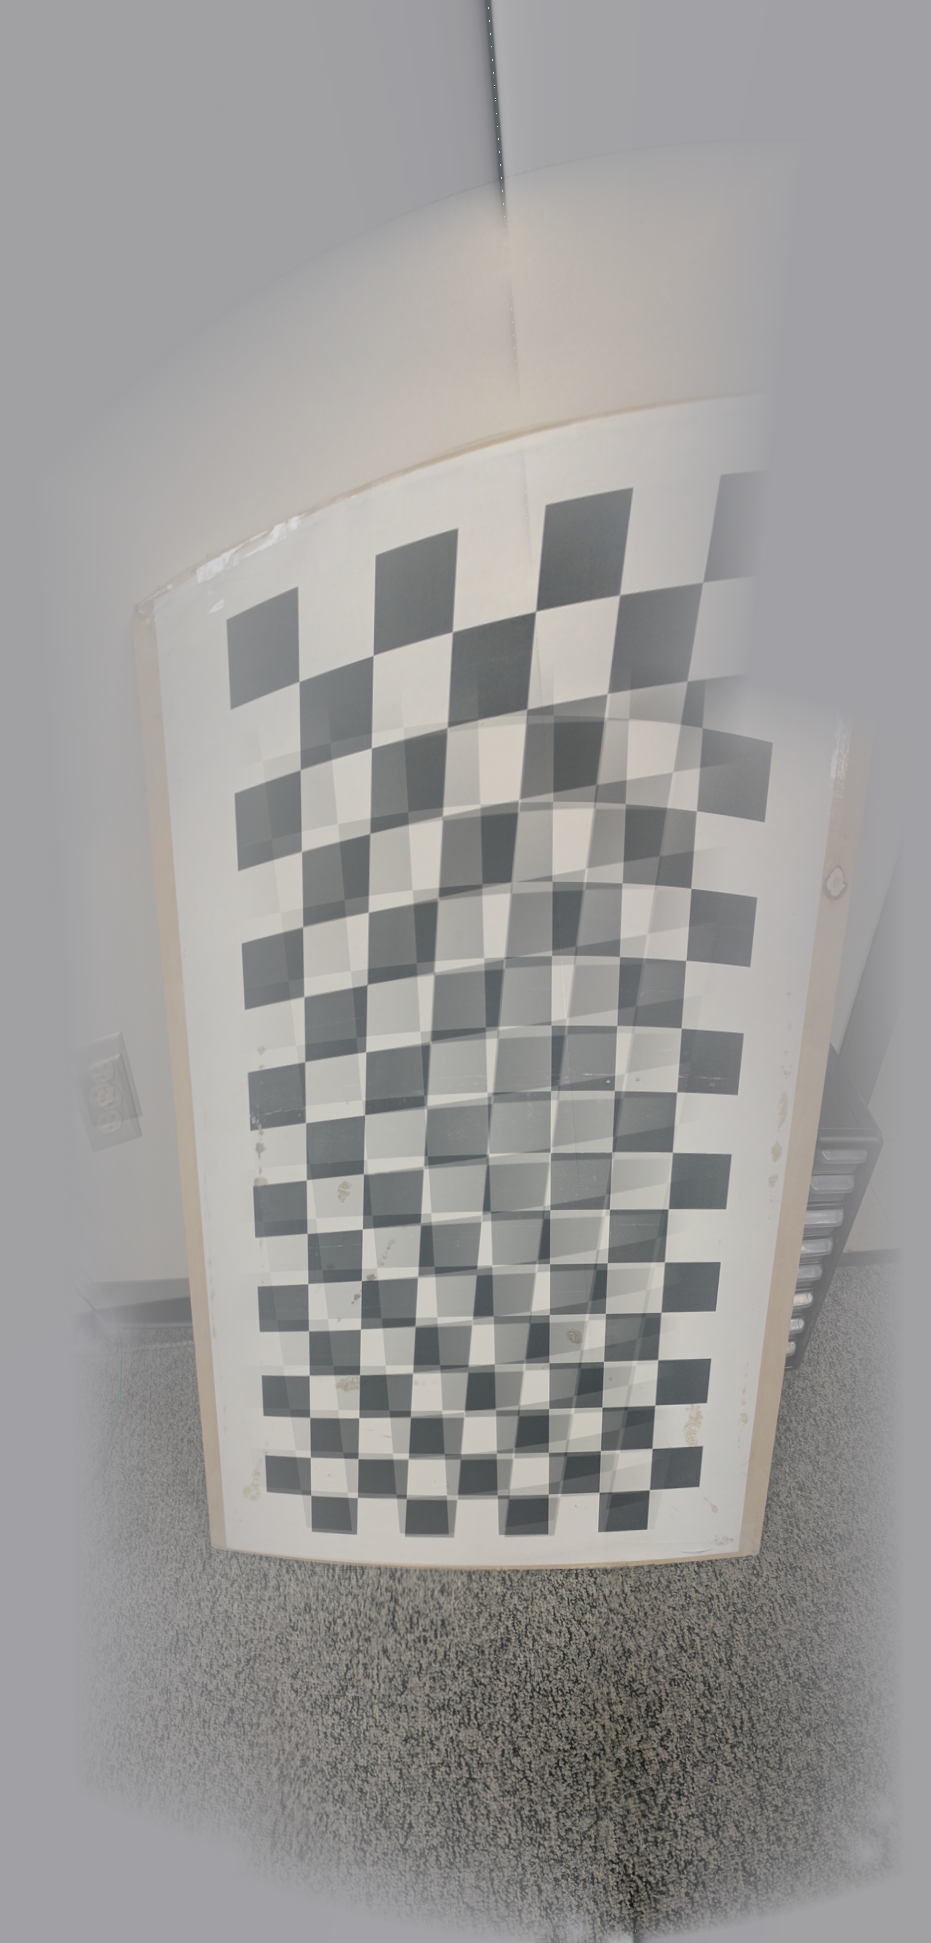
\includegraphics[width=\linewidth]{testset1.png}
\caption{Test set 1}
\label{fig_example}

\end{figure}
\begin{figure}[!t]
\centering
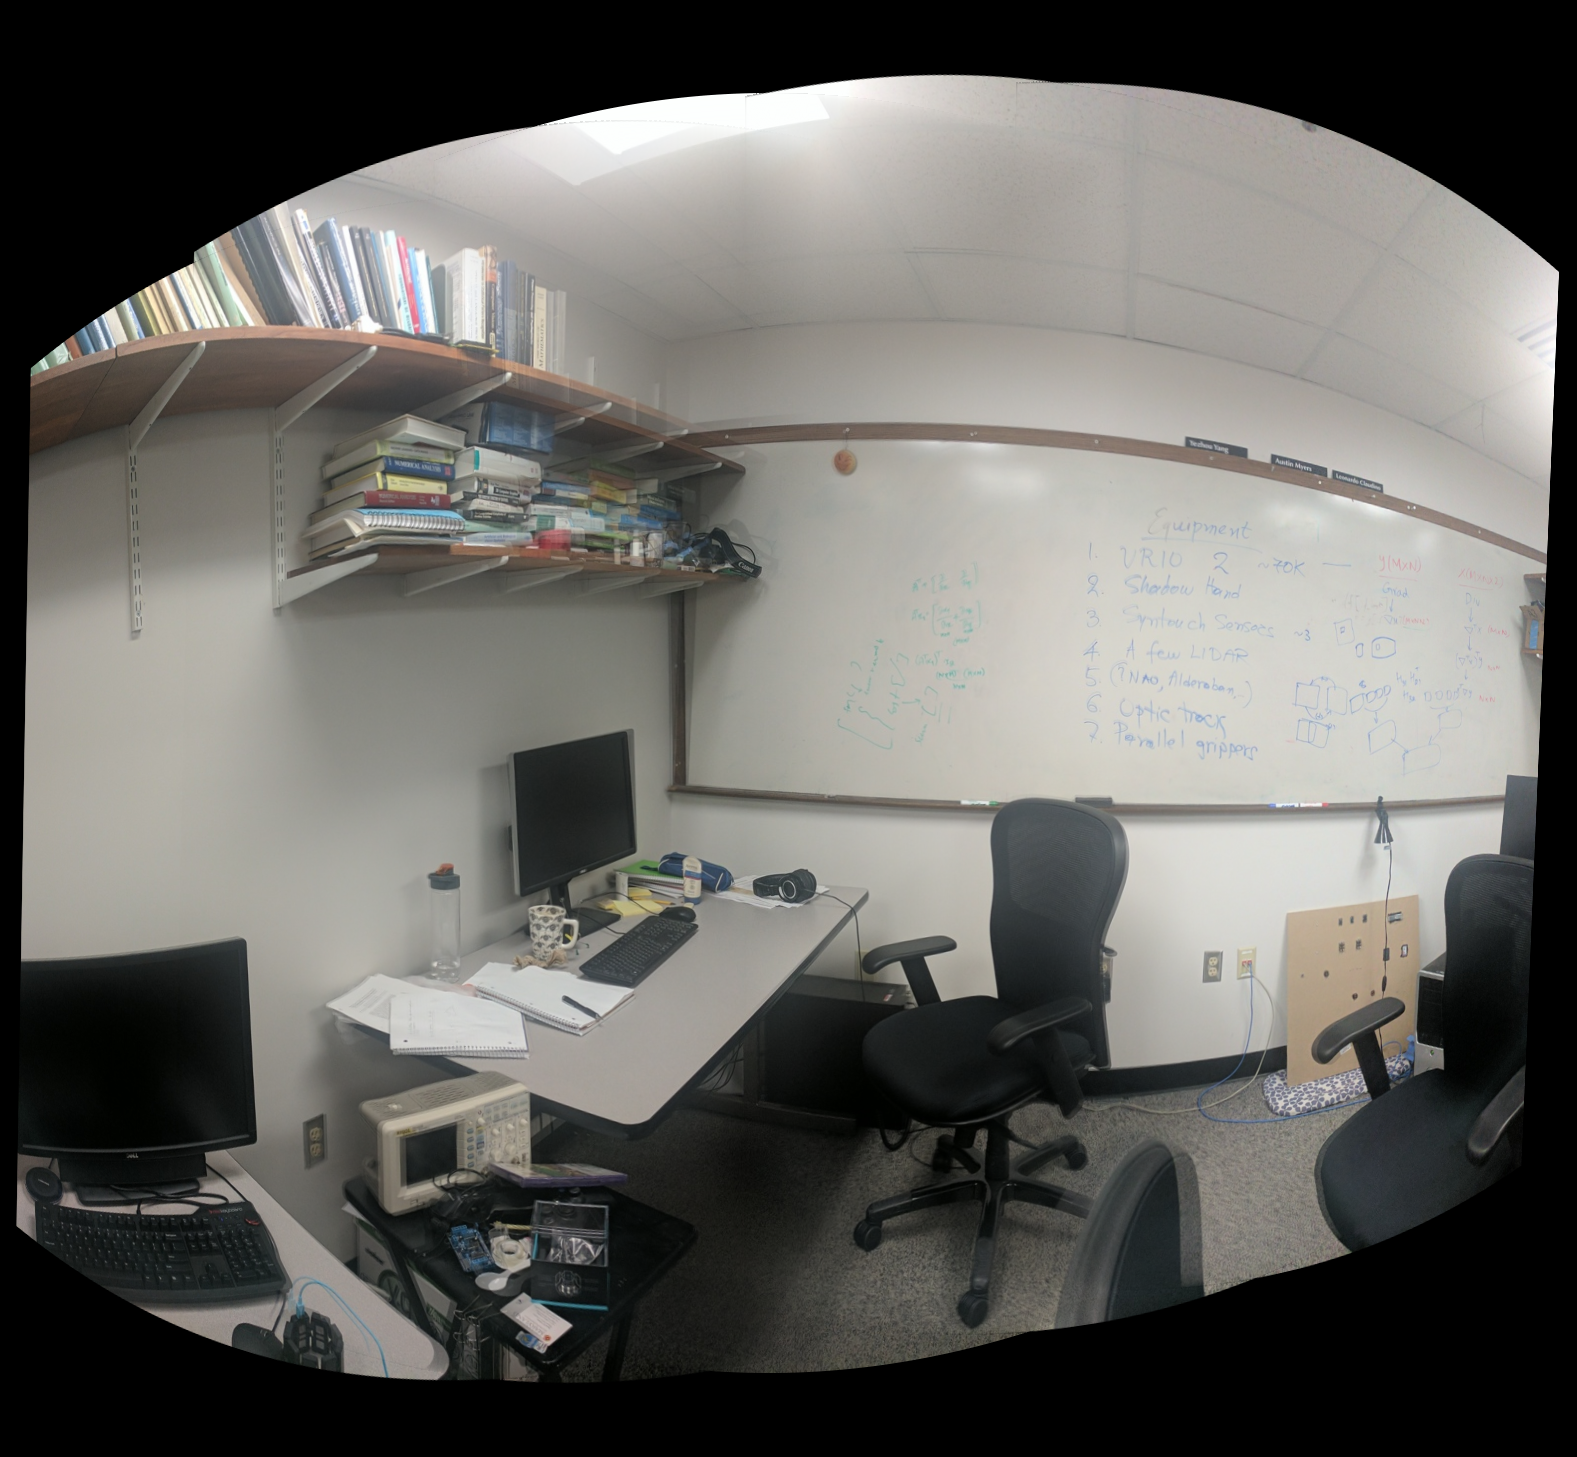
\includegraphics[width=\linewidth]{testset2.png}
\caption{Test set 2}
\label{fig_example}
\end{figure}

\begin{figure}[!t]
\centering
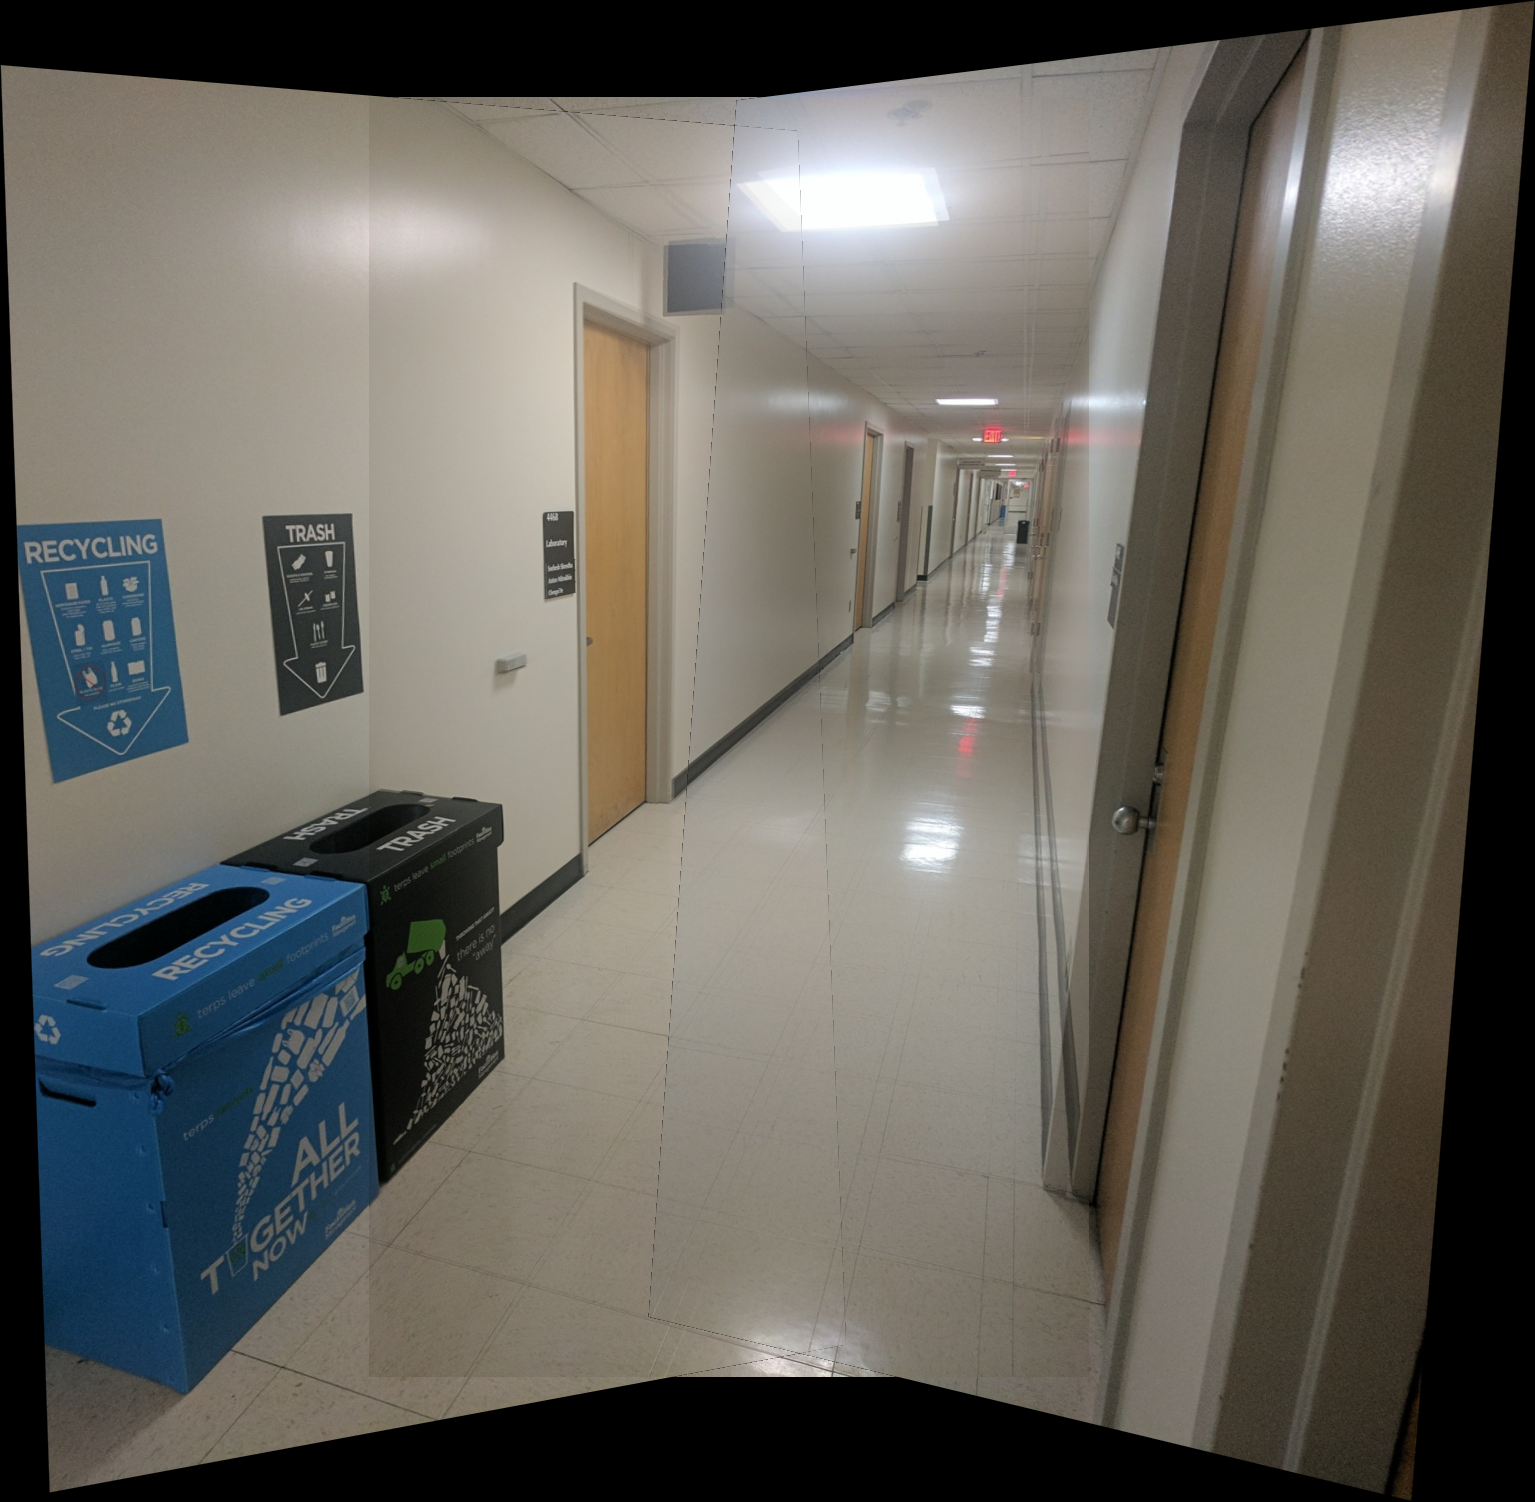
\includegraphics[width=\linewidth]{testset3.png}
\caption{Test set 3}
\label{fig_example}
\end{figure}

\begin{figure}[!t]
\centering
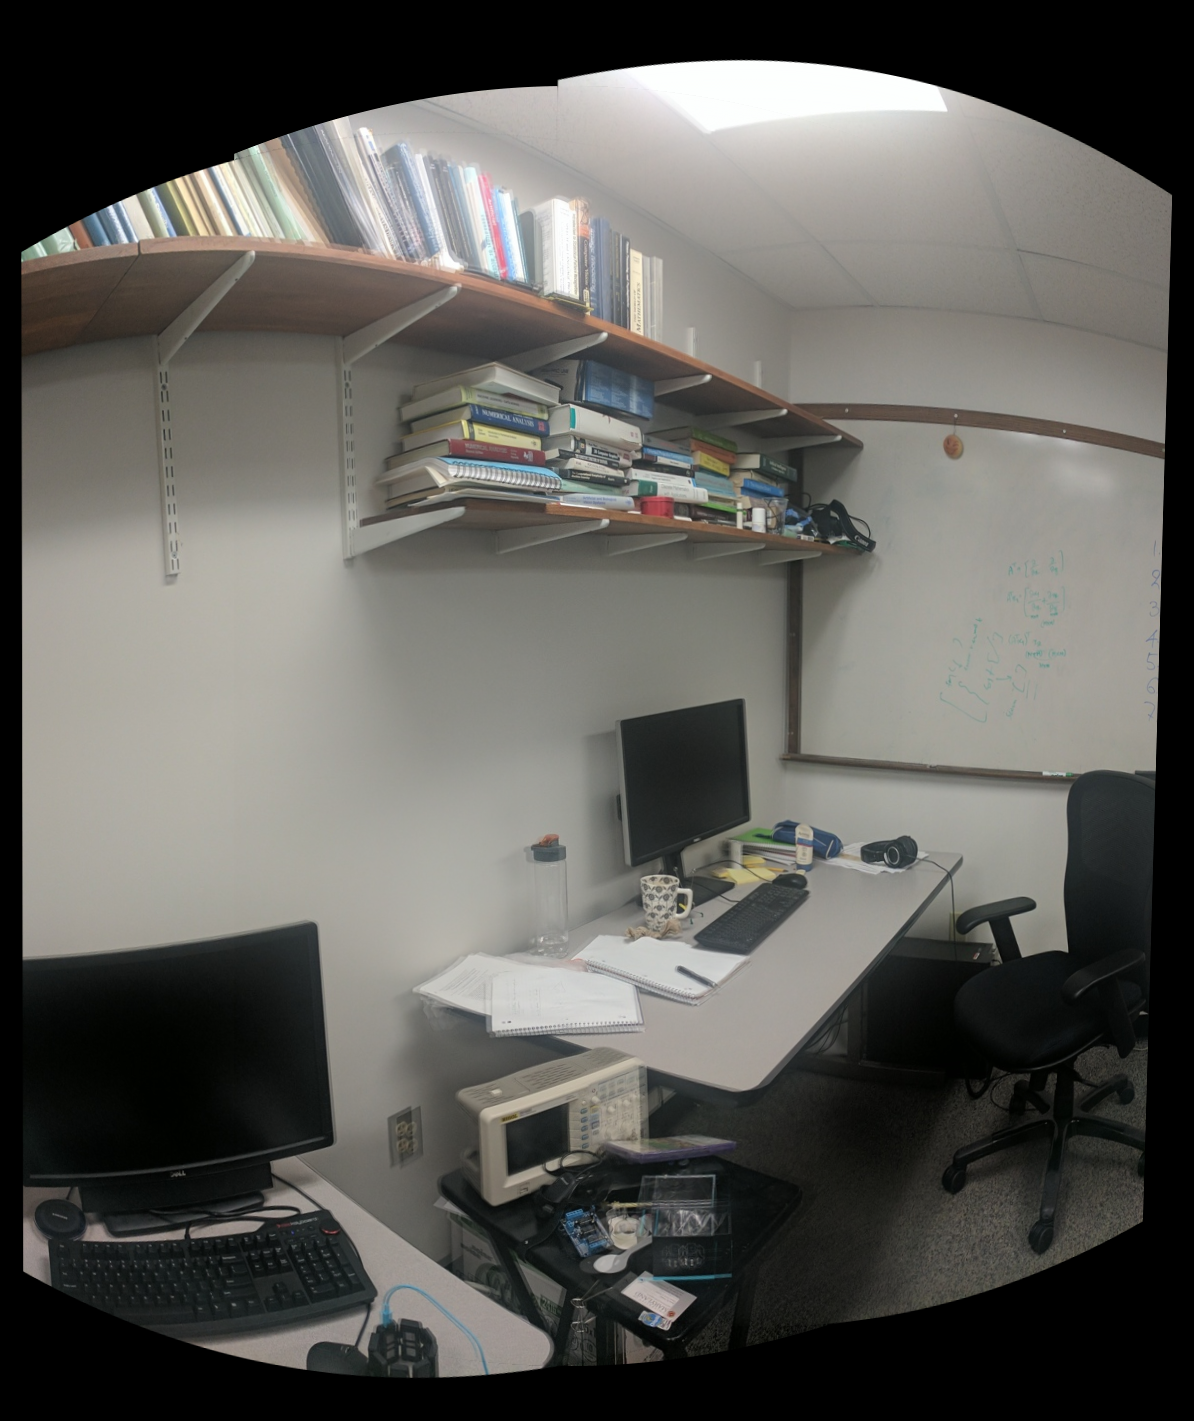
\includegraphics[width=\linewidth]{testset4.png}
\caption{Test set 4}
\label{fig_example}
\end{figure}

\begin{figure}[!t]
\centering
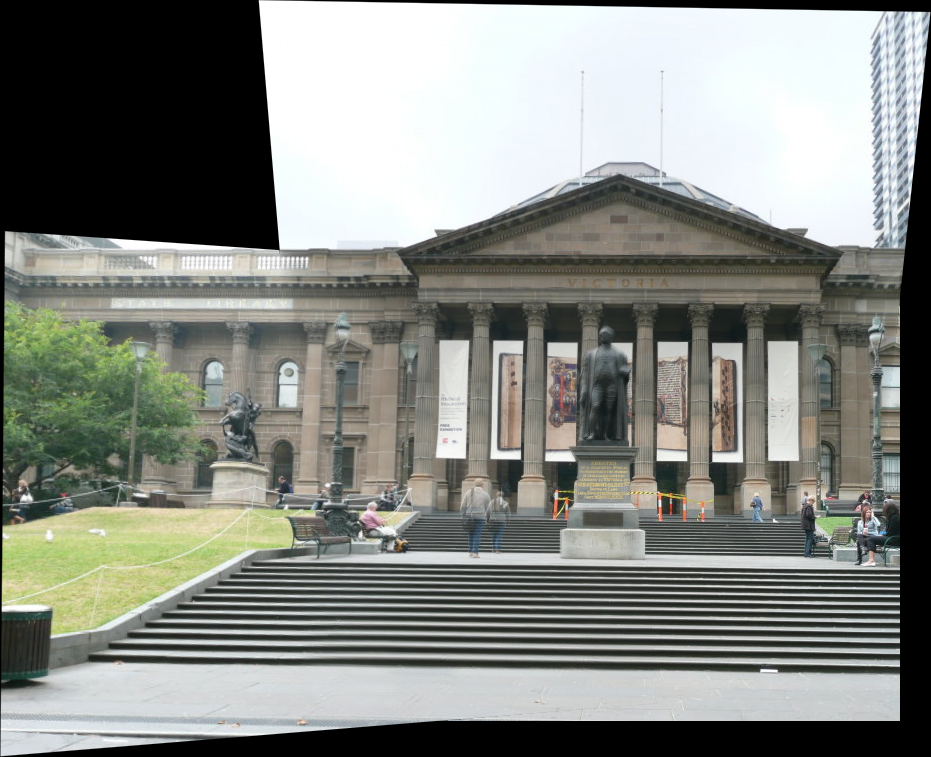
\includegraphics[width=\linewidth]{set1_feather.png}
\caption{Train set 1}
\label{fig_example}
\end{figure}

\begin{figure}[!t]
\centering
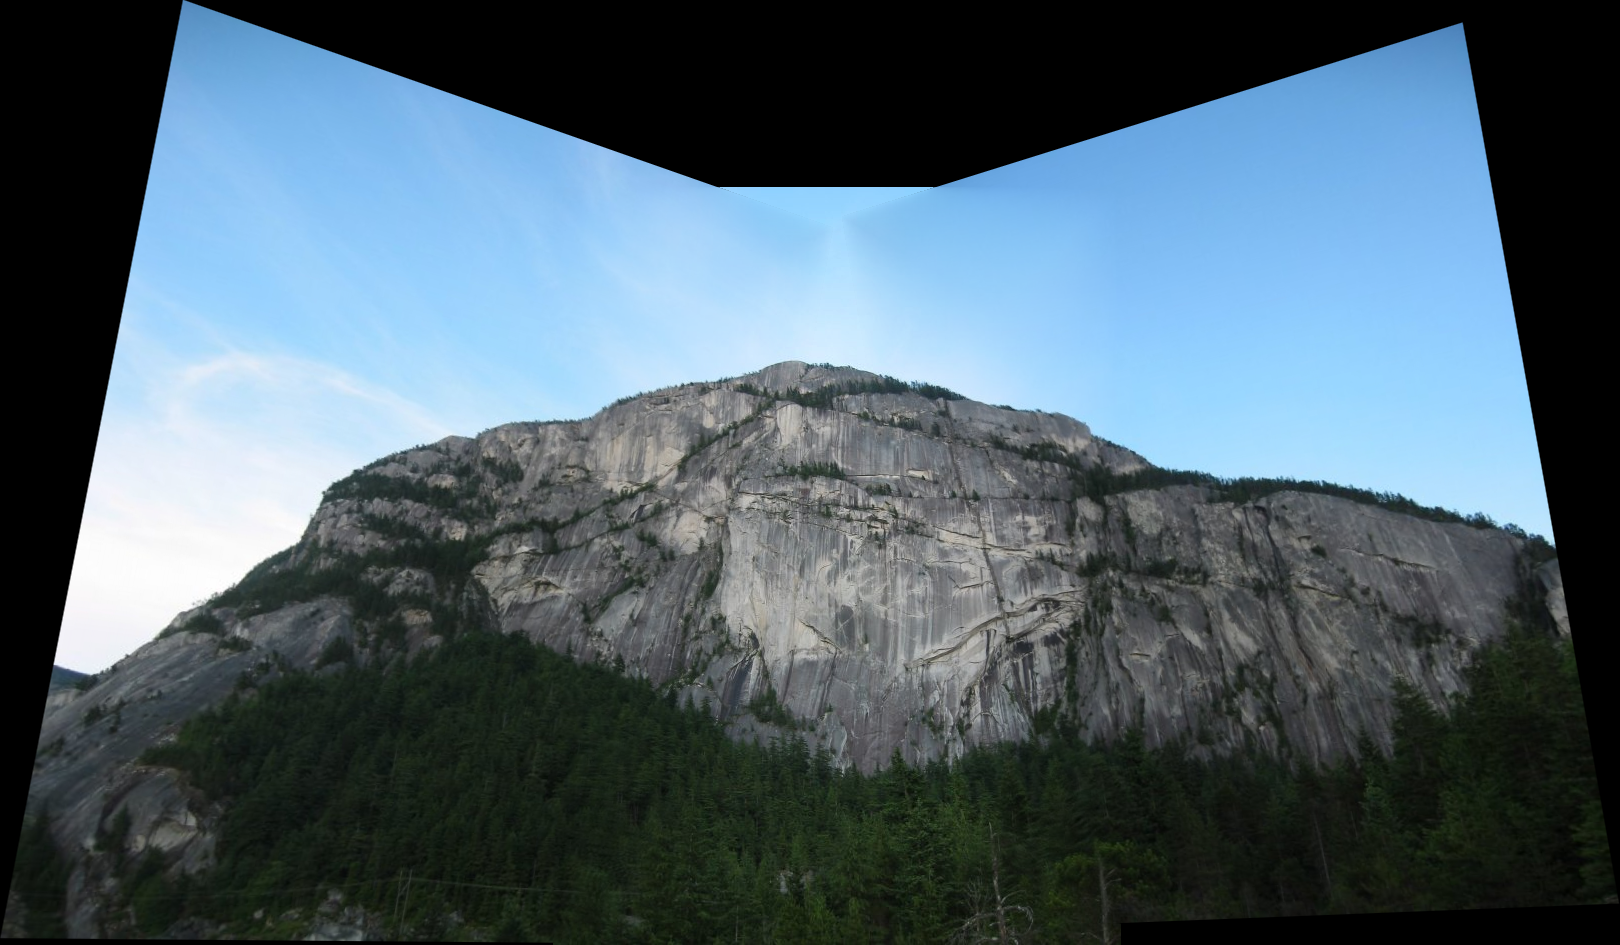
\includegraphics[width=\linewidth]{set2_feather.png}
\caption{Train set 2}
\label{fig_example}
\end{figure}

\subsection{Comments on final panoramas}
The final result panoramas are shown in Figure 6 and Figures 8 - 13.

Notice that some of the best stitching results are for test set 3,
train set 2, train set 1, and train set 3. These image sets share high density of good features 
that are distinct and non-repeating. There's also consistent brightness and contrast 
across the individual frames. Most of these have very nice overlap in the 30-50\% range.

We got a nice panorama from stitching the images of set 2, but images 5,6,9 in the set were cut out 
since they shared too little overlap with the reference middle image. We could fix this by 
carefully selecting the middle image or rearranging the order of the images.

We successfully ignored unrelated images in test set 4 due to rejecting images with too 
few inliers with the middle image, which happened to be in the scene that we want. We could 
have generated something worse if the middle image wasn't chosen correctly.

The checkerboard pattern in test set 1 has many similar-looking features due to the 
repetitiveness of the pattern. This causes the SSD ratio test to fail because the best 
match and second-best match look exactly the same, leading to sub-optimal alignment. 


% An example of a floating figure using the graphicx package.
% Note that \label must occur AFTER (or within) \caption.
% For figures, \caption should occur after the \includegraphics.
% Note that IEEEtran v1.7 and later has special internal code that
% is designed to preserve the operation of \label within \caption
% even when the captionsoff option is in effect. However, because
% of issues like this, it may be the safest practice to put all your
% \label just after \caption rather than within \caption{}.
%
% Reminder: the "draftcls" or "draftclsnofoot", not "draft", class
% option should be used if it is desired that the figures are to be
% displayed while in draft mode.
%
%\begin{figure}[!t]
%\centering
%\includegraphics[width=2.5in]{myfigure}
% where an .eps filename suffix will be assumed under latex, 
% and a .pdf suffix will be assumed for pdflatex; or what has been declared
% via \DeclareGraphicsExtensions.
%\caption{Simulation results for the network.}
%\label{fig_sim}
%\end{figure}

% Note that the IEEE typically puts floats only at the top, even when this
% results in a large percentage of a column being occupied by floats.


% An example of a double column floating figure using two subfigures.
% (The subfig.sty package must be loaded for this to work.)
% The subfigure \label commands are set within each subfloat command,
% and the \label for the overall figure must come after \caption.
% \hfil is used as a separator to get equal spacing.
% Watch out that the combined width of all the subfigures on a 
% line do not exceed the text width or a line break will occur.
%
%\begin{figure*}[!t]
%\centering
%\subfloat[Case I]{\includegraphics[width=2.5in]{box}%
%\label{fig_first_case}}
%\hfil
%\subfloat[Case II]{\includegraphics[width=2.5in]{box}%
%\label{fig_second_case}}
%\caption{Simulation results for the network.}
%\label{fig_sim}
%\end{figure*}
%
% Note that often IEEE papers with subfigures do not employ subfigure
% captions (using the optional argument to \subfloat[]), but instead will
% reference/describe all of them (a), (b), etc., within the main caption.
% Be aware that for subfig.sty to generate the (a), (b), etc., subfigure
% labels, the optional argument to \subfloat must be present. If a
% subcaption is not desired, just leave its contents blank,
% e.g., \subfloat[].


% An example of a floating table. Note that, for IEEE style tables, the
% \caption command should come BEFORE the table and, given that table
% captions serve much like titles, are usually capitalized except for words
% such as a, an, and, as, at, but, by, for, in, nor, of, on, or, the, to
% and up, which are usually not capitalized unless they are the first or
% last word of the caption. Table text will default to \footnotesize as
% the IEEE normally uses this smaller font for tables.
% The \label must come after \caption as always.
%
%\begin{table}[!t]
%% increase table row spacing, adjust to taste
%\renewcommand{\arraystretch}{1.3}
% if using array.sty, it might be a good idea to tweak the value of
% \extrarowheight as needed to properly center the text within the cells
%\caption{An Example of a Table}
%\label{table_example}
%\centering
%% Some packages, such as MDW tools, offer better commands for making tables
%% than the plain LaTeX2e tabular which is used here.
%\begin{tabular}{|c||c|}
%\hline
%One & Two\\
%\hline
%Three & Four\\
%\hline
%\end{tabular}
%\end{table}


% Note that the IEEE does not put floats in the very first column
% - or typically anywhere on the first page for that matter. Also,
% in-text middle ("here") positioning is typically not used, but it
% is allowed and encouraged for Computer Society conferences (but
% not Computer Society journals). Most IEEE journals/conferences use
% top floats exclusively. 
% Note that, LaTeX2e, unlike IEEE journals/conferences, places
% footnotes above bottom floats. This can be corrected via the
% \fnbelowfloat command of the stfloats package.




\section{Conclusion}
The conclusion goes here.




% conference papers do not normally have an appendix


% use section* for acknowledgment
\section*{Acknowledgment}


The authors would like to thank...





% trigger a \newpage just before the given reference
% number - used to balance the columns on the last page
% adjust value as needed - may need to be readjusted if
% the document is modified later
%\IEEEtriggeratref{8}
% The "triggered" command can be changed if desired:
%\IEEEtriggercmd{\enlargethispage{-5in}}

% references section

% can use a bibliography generated by BibTeX as a .bbl file
% BibTeX documentation can be easily obtained at:
% http://mirror.ctan.org/biblio/bibtex/contrib/doc/
% The IEEEtran BibTeX style support page is at:
% http://www.michaelshell.org/tex/ieeetran/bibtex/
%\bibliographystyle{IEEEtran}
% argument is your BibTeX string definitions and bibliography database(s)
%\bibliography{IEEEabrv,../bib/paper}
%
% <OR> manually copy in the resultant .bbl file
% set second argument of \begin to the number of references
% (used to reserve space for the reference number labels box)
\begin{thebibliography}{1}

\bibitem{IEEEhowto:kopka}
H.~Kopka and P.~W. Daly, \emph{A Guide to \LaTeX}, 3rd~ed.\hskip 1em plus
  0.5em minus 0.4em\relax Harlow, England: Addison-Wesley, 1999.

\end{thebibliography}




% that's all folks
\end{document}


